\documentclass[a4paper,12pt]{report}
\usepackage{graphicx} % for including images
\usepackage{hyperref} % for adding links
\hypersetup{
    colorlinks=true,       % keep the text itself colored instead of boxes
    linkcolor=black,       % color of internal links (sections, toc, etc.)
    citecolor=blue,        % citations (if any)
    urlcolor=blue,         % urls
    filecolor=blue,        % file links
    pdfborder={0 0 0}      % removes the red/green boxes completely
}
\usepackage{fancyhdr} % for customizing the header and footer
\usepackage{ragged2e} % for left-aligning text on the title page
\usepackage{multicol} % for placing signatures on the same line
\usepackage{float} % for [H] placement
\usepackage{svg}
% --- TikZ setup (add to preamble) ---
\usepackage{tikz}
\usetikzlibrary{arrows.meta, positioning, shapes.misc, shapes.geometric, fit, calc}
\tikzset{
  box/.style = {
    draw, rounded corners=2pt, align=center, minimum width=2.8cm, minimum height=1.2cm,
    inner sep=6pt, very thick, fill=white
  },
  smallbox/.style = {
    draw, rounded corners=2pt, align=center, minimum width=1.6cm, minimum height=0.9cm,
    inner sep=4pt, thick, fill=white
  },
  db/.style = {
    cylinder, draw, cylinder uses custom fill, cylinder body fill=white, shape border rotate=90,
    aspect=0.25, minimum height=1.2cm, minimum width=1.8cm, very thick
  },
  arrow/.style = {->, line width=1.1pt, >=Stealth, rounded corners},
  faint/.style = {opacity=0.85},
}
\pagestyle{fancy}
\fancyhf{}
\fancyhead[L]{Summer Practice Report}
\fancyfoot[C]{\thepage}

\begin{document}

% Title Page
\begin{titlepage}
    \centering
    \includegraphics[width=1\textwidth]{figures/cover_image.png} % Replace with actual cover image
    
    \vspace*{1cm}
    \Huge \textbf{SUMMER PRACTICE REPORT}
    \vspace{1.5cm}
    \LARGE \textbf{CENG400}
    
    \vfill
    \RaggedRight
    \large
    \textbf{STUDENT NAME:} Burak YILDIZ \\
    \textbf{ORGANIZATION NAME:} ODTÜ-DTX (ODTÜ Dijital Dönüşüm ve İnovasyon Merkezi) \\
    \textbf{ADDRESS:} BİLTİR Merkezi, Orta Doğu Teknik Üniversitesi, Dumlupınar Bulvarı 1, 06800 Çankaya/Ankara \\
    \textbf{START DATE:} 01.09.2025 \\
    \textbf{END DATE:} 26.09.2025 \\
    \textbf{TOTAL WORKING DAYS:} 20 \\
    \vfill

    \begin{multicols}{2}
        \raggedright \textbf{STUDENT’S SIGNATURE} \\
        \raggedleft \textbf{ORGANIZATION APPROVAL}
    \end{multicols}
    \vfill
\end{titlepage}

\tableofcontents
\newpage

% ---------------------------
\chapter{Introduction}
This report summarizes the summer practice I completed at ODTÜ-DTX (Dijital Dönüşüm ve İnovasyon Merkezi) between 01.09.2025 and 26.09.2025, under the supervision of Doç. Dr. Şeyda Ertekin.  
The practice was focused on improving my graduation project, a \textbf{Real-Time Location System (RTLS)} using BLE signals, ESP32 devices, and machine learning.  

The main objective was to advance the accuracy and robustness of indoor positioning systems by combining embedded hardware, cloud data pipelines, and advanced ML models.  
During this practice, I:
\begin{itemize}
    \item Programmed ESP32 boards to collect BLE RSSI data via ESP-NOW and uploaded readings to Firebase.
    \item Applied trilateration with path-loss models and compared its performance against ML-based approaches.
    \item Trained multiple ML models (kNN, Random Forest, SVM, XGBoost, Ensembles) on collected datasets.
    \item Performed feature engineering (differences, ratios, statistics) and applied Kalman filtering for noise reduction.
    \item Developed a frontend page for visualizing real-time ML-based predictions in the project’s web application.
    \item Delivered periodic reports, research summaries, and evaluations to my academic supervisor.
\end{itemize}

The following chapters explain the project phases, organizational environment, and my personal reflections.

% ---------------------------
\chapter{Information about the Project}

\section{Analysis Phase}
The project started with identifying the main challenges of indoor RTLS:
\begin{itemize}
    \item \textbf{Noisy RSSI signals:} BLE RSSI suffers from multipath fading and environmental interference.
    \item \textbf{Accuracy requirement:} Achieving sub-1 meter accuracy is difficult using RSSI alone.
    \item \textbf{Scalability:} The system must support many tags and scanners in real-time.
\end{itemize}

We explored multiple approaches: classical trilateration with path-loss models, fingerprinting with ML classifiers, and data smoothing via filters (Kalman).  
A data collection plan was prepared for two testbeds:
\begin{itemize}
    \item \textbf{Testbed A:} A $3 \times 4$ grid in a controlled lab environment, 1m $\times$ 1m cells, 60 samples per cell (total 720 samples).
    \item \textbf{Testbed B:} A $9 \times 12$ grid in a factory environment, 0.5m $\times$ 0.5m cells, 30 samples per cell (total 3240 samples).
\end{itemize}

% --- Figures for Analysis Phase ---
\begin{figure}[H]
    \centering
    \includegraphics[width=0.9\textwidth]{figures/layout_grid_testbedA.png}
    \caption{Testbed A layout and grid labeling (cell indices and anchor placement).}
    \label{fig:testbedA_layout}
\end{figure}

\begin{figure}[H]
    \centering
    \includegraphics[width=0.9\textwidth]{figures/layout_grid_testbedB.png}
    \caption{Testbed B layout (factory floor) with scanner (ESP32) anchor positions and walk path.}
    \label{fig:testbedB_layout}
\end{figure}

\begin{figure}[H]
    \centering
    \includegraphics[width=0.85\textwidth]{figures/rssi_noise_histogram.png}
    \caption{Typical RSSI distribution at a fixed cell showing variance and multipath-induced tails (motivation for filtering).}
    \label{fig:rssi_hist}
\end{figure}

\section{Design Phase}
The design phase focused on the end-to-end pipeline:
\begin{itemize}
    \item \textbf{Hardware:} 3 ESP32 scanners placed at key anchor points, configured with ESP-NOW for low-latency data collection.
    \item \textbf{Database:} Firebase Realtime Database as the central storage layer for RSSI readings.
    \item \textbf{Algorithms:} Both trilateration and ML models designed to process RSSI data.
    \item \textbf{Frontend:} Integration of a dashboard into the existing React-based webapp to visualize predictions and errors in real time.
\end{itemize}

Architectural diagrams were created to ensure modularity: hardware (data collection), software (data processing), ML (training + inference), and UI (visualization).  

% --- Figures for Design Phase ---
\begin{figure}[H]
  \centering
  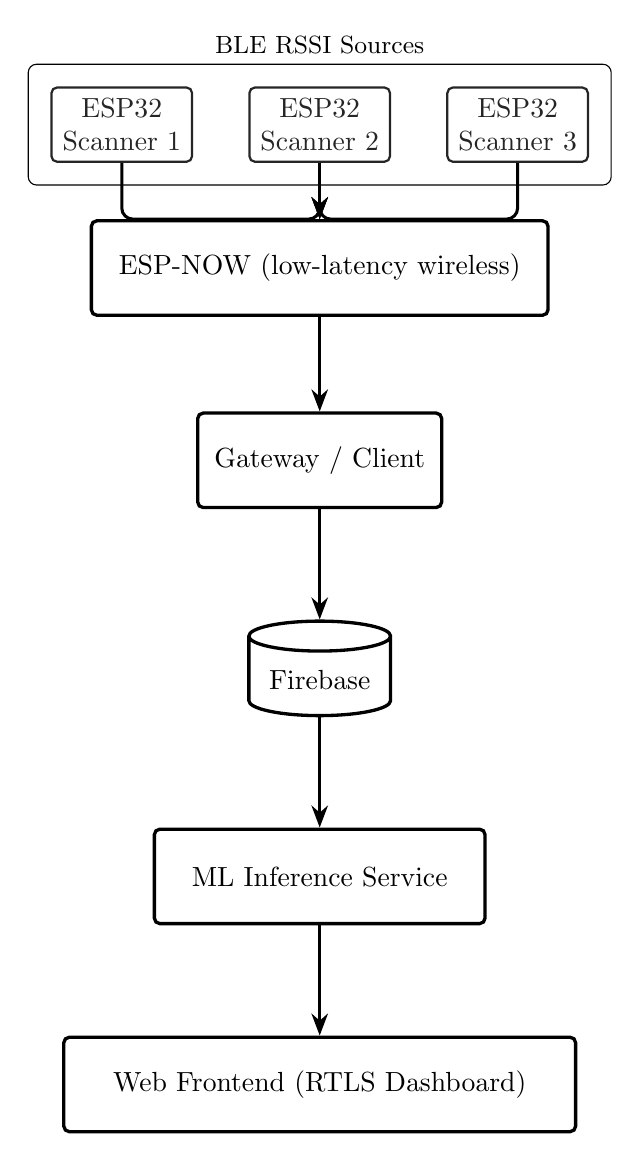
\begin{tikzpicture}[node distance=1.4cm and 1.0cm]
    % Row 1: ESP32 scanners (three small boxes grouped)
    \node[smallbox, faint] (s1) {ESP32\\Scanner 1};
    \node[smallbox, right=0.7cm of s1, faint] (s2) {ESP32\\Scanner 2};
    \node[smallbox, right=0.7cm of s2, faint] (s3) {ESP32\\Scanner 3};

    % ESP-NOW cloud-ish box (wide)
    \node[box, below=1.2cm of $(s1)!0.5!(s3)$, minimum width=5.8cm] (espnow) {ESP-NOW (low-latency wireless)};

    % Gateway/Client
    \node[box, below=1.2cm of espnow] (gateway) {Gateway / Client};

    % Firebase (DB cylinder)
    \node[db, below=1.4cm of gateway] (firebase) {Firebase};

    % ML Inference Service
    \node[box, below=1.4cm of firebase, minimum width=4.2cm] (ml) {ML Inference Service};

    % Web Frontend (wider to ensure content is fully inside)
    \node[box, below=1.4cm of ml, minimum width=6.5cm] (web) {Web Frontend (RTLS Dashboard)};

    % Group bracket for scanners for clarity (optional)
    \node[fit=(s1)(s2)(s3), draw, rounded corners=3pt, inner sep=8pt, label={[align=center]above:{\small BLE RSSI Sources}}] (scanGroup) {};

    % Arrows (route around text with gentle bends)
    \draw[arrow] (s1.south) |- ($(espnow.north)+(-1.9cm,0.0)$) -| (espnow.north);
    \draw[arrow] (s2.south) -- ($(espnow.north)$);
    \draw[arrow] (s3.south) |- ($(espnow.north)+(1.9cm,0.0)$) -| (espnow.north);

    \draw[arrow] (espnow.south) -- (gateway.north);
    \draw[arrow] (gateway.south) -- (firebase.north);
    \draw[arrow] (firebase.south) -- (ml.north);
    \draw[arrow] (ml.south) -- (web.north);

    % Side notes (optional, comment out if not needed)
    % \node[align=left, anchor=west] at ($(gateway.east)+(1.2cm,0)$) {\footnotesize
    %   \begin{tabular}{l}
    %   - Packet parsing \\
    %   - Authentication \\
    %   - Uplink buffering
    %   \end{tabular}};
  \end{tikzpicture}
  \caption{System architecture: ESP32 scanners $\rightarrow$ ESP-NOW $\rightarrow$ Gateway/Client $\rightarrow$ Firebase $\rightarrow$ ML inference service $\rightarrow$ Web frontend.}
  \label{fig:system_architecture}
\end{figure}

\begin{figure}[H]
  \centering
  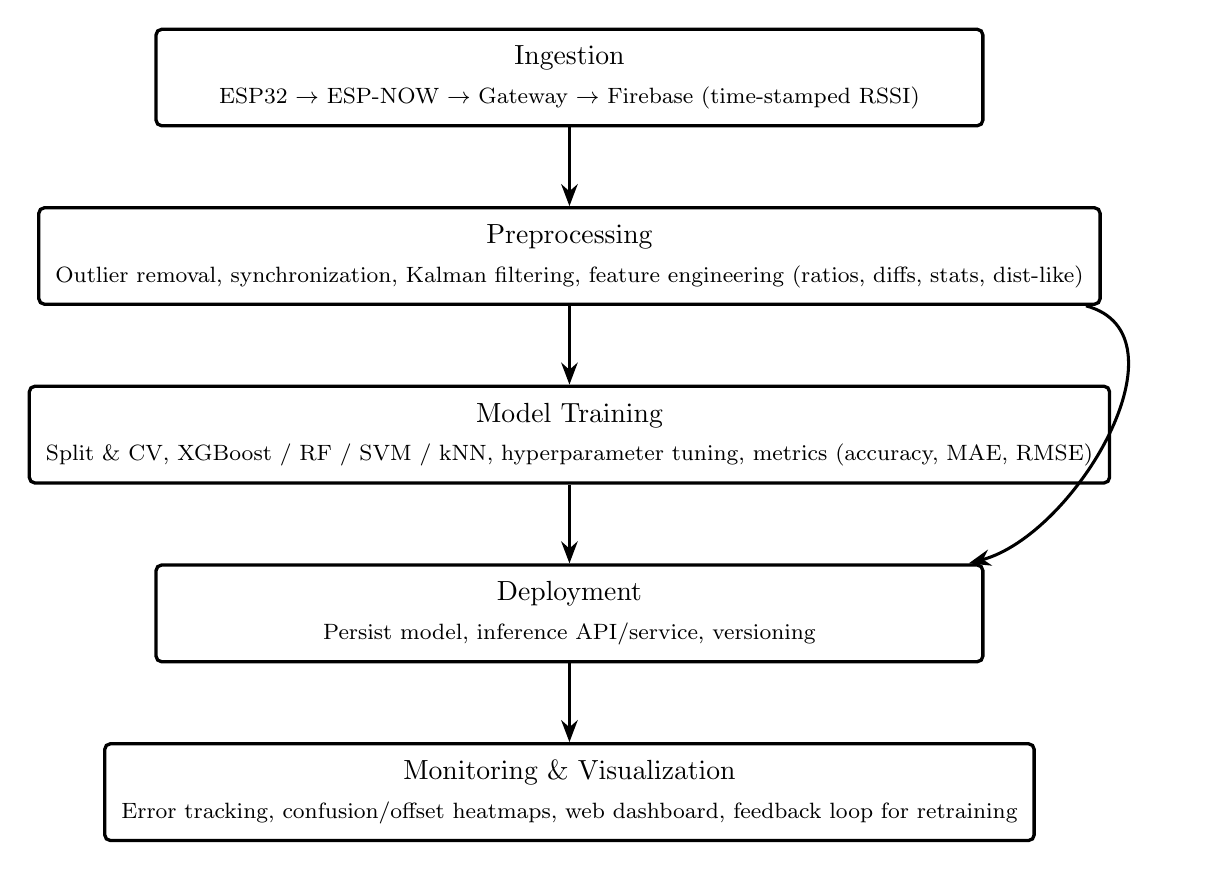
\begin{tikzpicture}[node distance=1.0cm and 1.0cm]
    % Pipeline stages laid out vertically and centered
    \node[box, minimum width=10.5cm] (ingest) {Ingestion\\[2pt]
      \footnotesize ESP32 $\rightarrow$ ESP-NOW $\rightarrow$ Gateway $\rightarrow$ Firebase (time-stamped RSSI)
    };

    \node[box, below=1.0cm of ingest, minimum width=10.5cm] (prep) {Preprocessing\\[2pt]
      \footnotesize Outlier removal, synchronization, Kalman filtering, feature engineering (ratios, diffs, stats, dist-like)
    };

    \node[box, below=1.0cm of prep, minimum width=10.5cm] (train) {Model Training\\[2pt]
      \footnotesize Split \& CV, XGBoost / RF / SVM / kNN, hyperparameter tuning, metrics (accuracy, MAE, RMSE)
    };

    \node[box, below=1.0cm of train, minimum width=10.5cm] (deploy) {Deployment\\[2pt]
      \footnotesize Persist model, inference API/service, versioning}
    ;

    \node[box, below=1.0cm of deploy, minimum width=10.5cm] (monitor) {Monitoring \& Visualization\\[2pt]
      \footnotesize Error tracking, confusion/offset heatmaps, web dashboard, feedback loop for retraining}
    ;

    % Arrows straight and clean, between box edges
    \draw[arrow] (ingest.south) -- (prep.north);
    \draw[arrow] (prep.south) -- (train.north);
    \draw[arrow] (train.south) -- (deploy.north);
    \draw[arrow] (deploy.south) -- (monitor.north);

    % Optional side tap for "live inference" from Preprocessing to Deployment
    \draw[arrow] ($(prep.south east)+(-0.2cm,0)$) to[out=-15, in=15] ($(deploy.north east)+(-0.2cm,0)$);

  \end{tikzpicture}
  \caption{Data pipeline and processing stages: ingestion, preprocessing (filtering \& feature engineering), model training, deployment, and monitoring.}
  \label{fig:data_pipeline}
\end{figure}

\begin{figure}[H]
    \centering
    \includegraphics[width=0.9\textwidth]{figures/firebase_schema.png}
    \caption{Firebase Realtime Database structure for RSSI samples, device metadata, and predictions.}
    \label{fig:firebase_schema}
\end{figure}

\begin{figure}[H]
    \centering
    \includegraphics[width=\textwidth]{figures/ui_wireframe.png}
    \caption{Frontend dashboard wireframe for real-time position visualization, confidence metrics, and error overlays.}
    \label{fig:ui_wireframe}
\end{figure}

\section{Implementation Phase}
The main implementation tasks were:
\begin{itemize}
    \item \textbf{ESP32 Programming:} Configured ESP32 WROOM-32 boards to scan BLE beacons, filter known MAC addresses, and transmit results via ESP-NOW.
    \item \textbf{Firebase Integration:} Implemented code to stream RSSI readings into structured JSON format.
    \item \textbf{ML Modeling:} Created pipelines for kNN, RF, SVM, and XGB, with feature engineering (ratios, differences, statistics, dist-like transforms).
    \item \textbf{Kalman Filtering:} Implemented an in-pipeline Kalman filter to reduce variance while preserving signal trends.
    \item \textbf{Frontend Extension:} Added an RTLS visualization panel to the web dashboard, showing real-time position predictions and error heatmaps.
\end{itemize}

% --- Figures for Implementation Phase (code + flows) ---
\begin{figure}[H]
    \centering
    \includegraphics[width=\textwidth]{figures/esp32_firmware_code.png}
    \caption{ESP32 firmware (ESP-NOW + BLE scan) code excerpt showing packet format and filtering logic.}
    \label{fig:esp32_code}
\end{figure}

\begin{figure}[H]
    \centering
    \includegraphics[width=\textwidth]{figures/firebase_ingest_code.png}
    \caption{Data ingestion snippet: pushing timestamped RSSI tuples to Firebase under session and cell keys.}
    \label{fig:firebase_code}
\end{figure}

\begin{figure}[H]
    \centering
    \includegraphics[width=\textwidth]{figures/ml_pipeline_code.png}
    \caption{ML training pipeline script: feature generation (ratios/diffs/stats), train/validation split, model registry.}
    \label{fig:ml_pipeline_code}
\end{figure}

\begin{figure}[H]
    \centering
    \includegraphics[width=0.95\textwidth]{figures/kalman_concept.png}
    \caption{Kalman filtering concept applied to RSSI streams: measurement vs. filtered estimate across time.}
    \label{fig:kalman_concept}
\end{figure}


\section{Testing Phase}
Testing included:
\begin{itemize}
    \item \textbf{Unit Testing:} Verified ESP32 firmware modules (BLE scanning, ESP-NOW transmission).
    \item \textbf{Dataset Testing:} Split datasets into 80/20 train-test for fair evaluation.
    \item \textbf{Cross-validation:} Used 5-fold CV for hyperparameter tuning of ML models.
    \item \textbf{Performance Metrics:} Accuracy, mean grid error, mean absolute error (MAE), and RMSE were tracked.
    \item \textbf{Visualization:} Confusion matrices and offset heatmaps used to diagnose spatial error distributions.
\end{itemize}

Results showed that ML-based fingerprinting with XGB and Random Forest achieved much higher accuracy than raw trilateration, especially when combined with feature engineering and Kalman filtering.

% --- Figures for Testing Phase (charts) ---
\begin{figure}[H]
    \centering
    \includegraphics[width=\textwidth]{figures/training_cv_curves.png}
    \caption{Cross-validation curve for XGBoost (max\_depth) and validation accuracy trends.}
    \label{fig:cv_curves}
\end{figure}

\begin{figure}[H]
    \centering
    \includegraphics[width=\textwidth]{figures/confusion_matrix.png}
    \caption{Confusion matrix over grid cells for the best model; darker diagonal indicates correct localizations.}
    \label{fig:confusion_matrix}
\end{figure}



% ---------------------------
\chapter{Organization}

\section{Organization and Structure}
ODTÜ-DTX (Dijital Dönüşüm ve İnovasyon Merkezi) is a research and innovation center at Middle East Technical University, focused on accelerating digital transformation in various domains.  
It operates in collaboration with faculty members and industry partners, providing an environment where academic research meets practical applications.  

The RTLS project was part of the center’s IoT and Industry 4.0 initiatives, supervised  by Doç. Dr. Şeyda Ertekin and technically supported by DTX staff.  
The team structure included:
\begin{itemize}
    \item \textbf{Supervisor:} Guidance on ML methodology, evaluation metrics, and research direction.
    \item \textbf{Other researchers:} Support on embedded systems and data pipelines.
    \item \textbf{Student Researcher (myself):} Responsible for implementation, experimentation, and reporting.
\end{itemize}



\section{Methodologies and Strategies Used in the Organization}
The organization follows a research-oriented but structured methodology:
\begin{itemize}
    \item \textbf{Agile-inspired workflow:} Weekly meetings to review progress and adapt research direction.
    \item \textbf{Experiment-driven development:} Hypothesize, implement, test, and compare ML and filtering approaches.
    \item \textbf{Continuous reporting:} Delivered reports and experimental results to the supervisor for feedback.
    \item \textbf{Toolset:} Python (scikit-learn, XGBoost, Firebase SDK), ESP-IDF/Arduino IDE for embedded programming, Firebase for cloud storage, React + TypeScript for frontend.
\end{itemize}

This methodology balanced research freedom with structured deliverables.

% ---------------------------
\chapter{Conclusion}
The summer practice at ODTÜ-DTX allowed me to deepen my expertise in embedded systems, IoT data pipelines, and ML for real-time localization.  
Key achievements include:
\begin{itemize}
    \item Successfully built a complete RTLS pipeline: ESP32 scanners $\rightarrow$ Firebase $\rightarrow$ ML pipeline $\rightarrow$ frontend visualization.
    \item Demonstrated that ML fingerprinting outperforms trilateration in noisy indoor environments.
    \item Validated that Kalman filtering can reduce RSSI noise and improve prediction stability.
    \item Delivered reproducible datasets, trained models, and visualization dashboards.
\end{itemize}

This practice provided me with hands-on experience in both hardware and ML, preparing me for future research and industrial projects in IoT and smart factory domains.


\end{document}